\documentclass[10pt,a4paper]{article}
\usepackage[utf8]{inputenc}
\usepackage[english]{babel}
\usepackage{amsmath}
\usepackage{amsfonts}
\usepackage{amssymb}
\usepackage{graphicx}
\usepackage{tikz}
\usepackage{lipsum}
\usepackage[left=2cm,right=2cm,top=2cm,bottom=2cm]{geometry}
\author{Ludovic}
\title{Quelques exemples avec tikz}
\begin{document}
\maketitle



\begin{center}
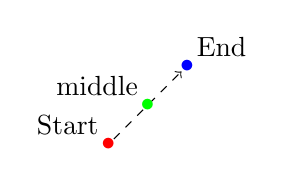
\begin{tikzpicture}
\coordinate (D) at (0, 0);

\draw [->, style = dashed, 
       shorten >= 1mm, 
       shorten <= 1mm] 
       (0, 0) node[color = red] (A) {$\bullet$} --
       (1, 1) node[color = blue] (B)  {$\bullet$};
\draw (A) node[above left] {Start};
\draw (B) node[above right] {End};
\path (A) -- (B) node[pos = .5] (C) {};
\draw (C) node [color = green] {$\bullet$};
\draw (C) node[above left] {middle};
\end{tikzpicture}
\end{center}


\begin{center}
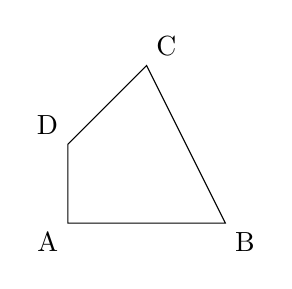
\begin{tikzpicture}
\coordinate (A) at (0, 0);
\coordinate (B) at (2, 0);
\coordinate (C) at (1, 2);
\coordinate (D) at (0, 1);
\draw[] (A) -- (B) -- (C) -- (D) -- cycle; 
\draw (A) node [below left] {A};
\draw (B) node [below right] {B};
\draw (C) node [above right] {C};
\draw (D) node [above left] {D};
\end{tikzpicture}
\end{center}



\end{document}